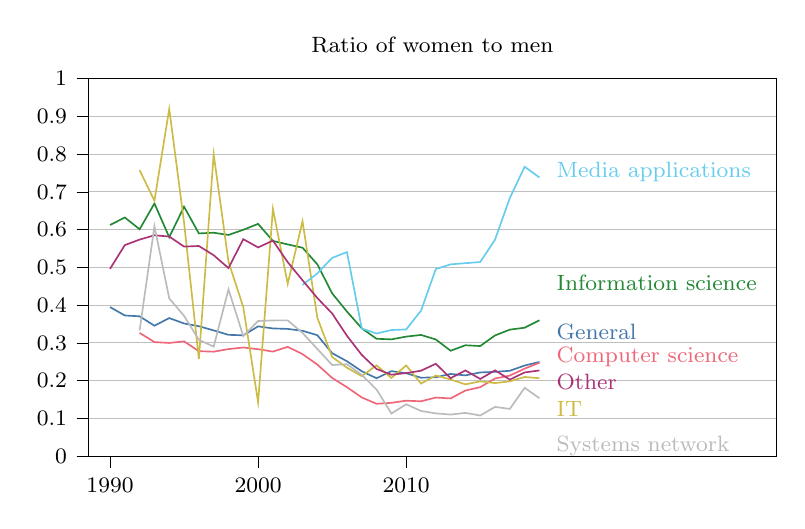
\begin{tikzpicture}[align=left,
every node/.style={font=\footnotesize}]
% This file was created with tikzplotlib v0.9.17.
\definecolor{color0}{rgb}{0.266666666666667,0.466666666666667,0.666666666666667}
\definecolor{color1}{rgb}{0.933333333333333,0.4,0.466666666666667}
\definecolor{color2}{rgb}{0.133333333333333,0.533333333333333,0.2}
\definecolor{color3}{rgb}{0.8,0.733333333333333,0.266666666666667}
\definecolor{color4}{rgb}{0.4,0.8,0.933333333333333}
\definecolor{color5}{rgb}{0.666666666666667,0.2,0.466666666666667}

\begin{axis}[
height=6.376357092455836cm,
tick align=outside,
tick pos=left,
title={Ratio of women to men},
width=10.317162499999998cm,
x grid style={white!69.0196078431373!black},
xmin=1988.55, xmax=2035,
xtick style={color=black},
xtick={1990,2000,2010},
xticklabels={\(\displaystyle 1990\),\(\displaystyle 2000\),\(\displaystyle 2010\)},
ymajorgrids,
ymin=0, ymax=1,
ytick style={color=black},
ytick={0,0.1,0.2,0.3,0.4,0.5,0.6,0.7,0.8,0.9,1},
yticklabels={
  \(\displaystyle 0\),
  \(\displaystyle 0.1\),
  \(\displaystyle 0.2\),
  \(\displaystyle 0.3\),
  \(\displaystyle 0.4\),
  \(\displaystyle 0.5\),
  \(\displaystyle 0.6\),
  \(\displaystyle 0.7\),
  \(\displaystyle 0.8\),
  \(\displaystyle 0.9\),
  \(\displaystyle 1\)
}
]
\addplot [semithick, color0]
table {%
1990 0.394967913627625
1991 0.37271773815155
1992 0.370465278625488
1993 0.345574140548706
1994 0.365840792655945
1995 0.351528167724609
1996 0.344272255897522
1997 0.3332200050354
1998 0.321436882019043
1999 0.320170640945435
2000 0.343914747238159
2001 0.338396310806274
2002 0.337104439735413
2003 0.332112669944763
2004 0.320477366447449
2005 0.272923469543457
2006 0.251452445983887
2007 0.225056648254395
2008 0.206436157226562
2009 0.225293636322021
2010 0.219744563102722
2011 0.207880258560181
2012 0.208938837051392
2013 0.217817306518555
2014 0.214048385620117
2015 0.221825838088989
2016 0.223389029502869
2017 0.226261734962463
2018 0.240228176116943
2019 0.249625205993652
};
\addplot [semithick, color1]
table {%
1992 0.326546549797058
1993 0.302248120307922
1994 0.299922227859497
1995 0.304198503494263
1996 0.278148174285889
1997 0.276795387268066
1998 0.283663749694824
1999 0.287935495376587
2000 0.283360481262207
2001 0.276973247528076
2002 0.289675116539001
2003 0.270382165908813
2004 0.242696404457092
2005 0.207340955734253
2006 0.182779669761658
2007 0.155608177185059
2008 0.138748645782471
2009 0.141365051269531
2010 0.146981954574585
2011 0.145420074462891
2012 0.155357122421265
2013 0.152976155281067
2014 0.173902153968811
2015 0.182833433151245
2016 0.205791473388672
2017 0.213488936424255
2018 0.231927156448364
2019 0.247621655464172
};
\addplot [semithick, color2]
table {%
1990 0.612352132797241
1991 0.632269382476807
1992 0.601075768470764
1993 0.669402599334717
1994 0.580039978027344
1995 0.660787582397461
1996 0.590057373046875
1997 0.591881036758423
1998 0.586007714271545
1999 0.599660754203796
2000 0.615333080291748
2001 0.570116519927979
2002 0.560919523239136
2003 0.552210807800293
2004 0.508236169815063
2005 0.431290030479431
2006 0.383183717727661
2007 0.338664650917053
2008 0.311026573181152
2009 0.309437870979309
2010 0.316780805587769
2011 0.321109294891357
2012 0.309195876121521
2013 0.279330730438232
2014 0.293806076049805
2015 0.291763782501221
2016 0.319848775863647
2017 0.335242509841919
2018 0.340254306793213
2019 0.36008358001709
};
\addplot [semithick, color3]
table {%
1992 0.757575750350952
1993 0.676470518112183
1994 0.920000076293945
1995 0.61904764175415
1996 0.257142901420593
1997 0.799999952316284
1998 0.515151500701904
1999 0.394736886024475
2000 0.142857193946838
2001 0.655172348022461
2002 0.45652174949646
2003 0.62232780456543
2004 0.366598844528198
2005 0.262847542762756
2006 0.234259247779846
2007 0.212081432342529
2008 0.240674495697021
2009 0.207284450531006
2010 0.240404009819031
2011 0.192297101020813
2012 0.213742017745972
2013 0.20320463180542
2014 0.190322637557983
2015 0.198224902153015
2016 0.193636417388916
2017 0.198331236839294
2018 0.209817886352539
2019 0.206441879272461
};
\addplot [semithick, color4]
table {%
2003 0.453731298446655
2004 0.484068632125854
2005 0.525307774543762
2006 0.540609121322632
2007 0.338213801383972
2008 0.324988007545471
2009 0.334102392196655
2010 0.335807085037231
2011 0.385281324386597
2012 0.495648741722107
2013 0.508133172988892
2015 0.514325976371765
2016 0.573572158813477
2017 0.684032797813416
2018 0.766576766967773
2019 0.73820161819458
};
\addplot [semithick, color5]
table {%
1990 0.496227502822876
1991 0.559025049209595
1992 0.573730945587158
1993 0.585096597671509
1994 0.581833839416504
1995 0.555163264274597
1996 0.556740999221802
1997 0.532289624214172
1998 0.498251676559448
1999 0.574840784072876
2000 0.552963495254517
2001 0.571029543876648
2002 0.514033436775208
2003 0.465948820114136
2004 0.418907046318054
2005 0.378113269805908
2006 0.318900346755981
2007 0.268292665481567
2008 0.230987310409546
2009 0.215844392776489
2010 0.220114707946777
2011 0.22640061378479
2012 0.24478816986084
2013 0.206656098365784
2014 0.22716224193573
2015 0.20456874370575
2016 0.227431774139404
2017 0.202842831611633
2018 0.221844434738159
2019 0.22710919380188
};
\addplot [semithick, white!73.3333333333333!black]
table {%
1992 0.333333373069763
1993 0.609375
1994 0.41791045665741
1995 0.371794939041138
1996 0.308411240577698
1997 0.290123462677002
1998 0.441913366317749
1999 0.318181753158569
2000 0.358090162277222
2001 0.359615325927734
2002 0.359693884849548
2003 0.326538920402527
2005 0.241577386856079
2006 0.243598818778992
2007 0.215324878692627
2008 0.176638126373291
2009 0.113035559654236
2010 0.1375333070755
2011 0.119799137115479
2012 0.11332905292511
2013 0.110236167907715
2014 0.114686965942383
2015 0.107761025428772
2016 0.130511522293091
2017 0.12526535987854
2018 0.181153535842896
2019 0.153496861457825
};
\draw (axis cs:2019.5,0.309625187406297) node[
  anchor=base west,
  text=color0,
  rotate=0.0
]{General};
\draw (axis cs:2019.5,0.247621668370155) node[
  anchor=base west,
  text=color1,
  rotate=0.0
]{Computer science};
\draw (axis cs:2019.5,0.44008353221957) node[
  anchor=base west,
  text=color2,
  rotate=0.0
]{Information science};
\draw (axis cs:2019.5,0.106441922563418) node[
  anchor=base west,
  text=color3,
  rotate=0.0
]{IT};
\draw (axis cs:2019.5,0.738201689021361) node[
  anchor=base west,
  text=color4,
  rotate=0.0
]{Media applications};
\draw (axis cs:2019.5,0.177109156337465) node[
  anchor=base west,
  text=color5,
  rotate=0.0
]{Other};
\draw (axis cs:2019.5,0.0134968210717529) node[
  anchor=base west,
  text=white!73.3333333333333!black,
  rotate=0.0
]{Systems network};
\end{axis}



\end{tikzpicture}
